\documentclass{classrep}
\usepackage[utf8]{inputenc}

\usepackage{listings}
\usepackage{graphicx}
\usepackage[none]{hyphenat}
\usepackage{float}
\usepackage{geometry}
\usepackage{lipsum}
\usepackage{afterpage}

\studycycle{Informatyka, studia niestacjonarne}

\coursesemester{V}

\coursename{Sztuczna inteligencja i systemy ekspertowe}
\courseyear{2018/2019}

\courseteacher{dr inż. Przemysław Nowak}
\coursegroup{niedziela, 17:15}

\author{
  \studentinfo{Marcin Pajkowski}{211968} \and
  \studentinfo{Rafał Warda}{214067}
}

\title{Przeszukiwanie przestrzeni stanów}

\begin{document}

\begin{titlepage}
\maketitle
\thispagestyle{empty}
\end{titlepage}

\section{Cel}

Implementacja grafowych algorytmów przeszukiwania przestrzeni stanów,
porównanie metod ślepych i heurystycznych na przykładzie układanki
``piętnastka''.

\section{Wprowadzenie}

\subsection{O grze ``piętnastka''}

``Piętnastka'' jest grą z serii łamigłówek logicznych. Układanka posiada
wymiar MxN (najczęściej są to układy o równych wymiarach - 4x4 lub 3x3).
Jedno pole jest zawsze wolne. Gracz wykonuje ruchy przemieszczając
klocki z wykorzystaniem wolnego pola. Elementy układanki mogą
reprezentować liczby - wówczas zadaniem gracza jest ułożenie elementów w
odpowiednim szeregu.

\subsection{Złożoność problemu i rozwiązywalność}

Ilość stanów każdej układanki można wyznaczyć za pomocą wzoru:
\[ iloscStanów = iloscPól! \] Dla układanki 4x4 będzie to liczba
\[ 16! = 2.0922789888 * 10^{13} \] Jednakże nie wszystkie układy są
rozwiązywalne. Możemy je podzielić na parzyste i nieparzyste - co
oznacza, że do uzyskania stanu wzorcowego należy wykonać parzystą lub
nieparzystą liczbę ruchów. Wszystkie układy pochodzące poprzez
przesuwanie klocków w obrębie wolnego pola, począwszy od układu
docelowego, są układami parzystymi.

\subsection{Grafowa reprezentacja przestrzeni
stanów}

Grafem nazywamy obiekt matematyczny składający się z niepustego zbioru
wierzchołków W i zbioru krawędzi K łączącego niektóre z tych
wierzchołków {[}1{]}. Graf może świetnie posłużyć do zapisu przebiegu
gry ``piętnastka''. Za wierzchołki grafu można przyjąć kolejne stany
planszy układanki, a krawędzie można zdefiniować jako kierunek
przesunięcia wolnego pola (tj. zamiany wolnego pola z elementem
znajdującym się względem niego nad nim, pod nim, z jego lewej lub prawej
strony).

\subsection{Metody przeszukiwania przestrzeni stanów}

Do przeszukiwania grafu przestrzeni stanów w celu znalezienia
rozwiązania układanki zostaną zaprezentowane następujące podejścia:

\begin{itemize}
\item
  Metody ślepe (klasyczne):

  \begin{itemize}
  \item
    breadth-first search (BFS)
  \item
    depth-first search (DFS)
  \end{itemize}
\item
  Metody oparte o heurystyki:

  \begin{itemize}
  \item
    algorytm A*
  \end{itemize}
\end{itemize}

Algorytmy klasyczne jako dodatkowy parametr przyjmują \textbf{porządek
przeszukiwania}, zaś algorytm A* do przyspieszenia procesu
przeszukiwania wykorzystuje \textbf{metryki} - zostaną zaprezentowane
metryka Hamminga oraz Manhattan (inaczej metryka taxicab lub metryka
miejska).

Algorytm \textbf{BFS} przeszukuje graf \textbf{wszerz} - w pierwszej
kolejności odwiedzany jest stan początkowy, następnie sąsiedzi stanu
początkowego, dalej sąsiedzi sąsiadów rozwiniętych w poprzednich
iteracjach - do momentu znalezienia stanu wzorcowego.

Inny algorytm z tej grupy - \textbf{DFS} przeszukuje graf \textbf{w
głąb} - w pierwszej kolejności odwiedzany jest stan początkowy,
następnie sąsiedzi stanu początkowego (zgodnie z podanym wcześniej
porządkiem przeszukiwania). Następnie odwiedzany jest stan-dziecko
będący blabla (TODO)

Zasadniczą różnicą między tymi dwoma podejściami jest to, że klasyczne
algorytmy poszukują rozwiązanie zgodnie z określonym porządkiem i nie
próbują aproksymować zasadności następnego ruchu. W praktyce nie musi to
oznaczać, że algorytmy klasyczne są nieoptymalne - przykładowo algorytm
BFS znajduje zawsze rozwiazanie optymalne.

\section{Implementacja}

Program został napisany w technologii C++ 17 z wykorzystaniem biblioteki
Google Test wspierającej testy jednostkowe. Stan układanki przedstawiony
jest jako klasa State. Klasa ta zawiera jednowymiarową tablicę o
wielkości NxM - układanka została zrzutowana na jeden wymiar celem
zredukowania zjawiska \emph{cache miss}. Informacje o rzeczywystych
wymiarach zapisane są w atrybutach klasy. Do zrealizowania
poszczególnych metod przeszukiwania przestrzeni stanów posłużono się
algorytmami i strukturami danych dostępnymi w bibliotece STL języka C++.

\section{Materiały i metody}
Do zrealizowania zadania zostały użyte następujące programy i skrypty wspomagające dostarczone razem z kartą
przedmiotu:
 \begin{itemize}
   \item
   Generator układanek,
   \item
   Walidator układanek,
   \item
   Wizualizator układanek,
   \item
   Skrypt uruchamiające program przeszukujący w trybie wsadowym (powłoka bash),
   \item
   Skrypt ekstraktujący dane wygenerowane podczas przeszukiwania (powłoka bash).
\end{itemize}
Do stworzenia pliku binarnego solvera z kodu źródłowego C++ użyto kompilatora Clang z pakietu LLVM.
Prezentacja graficzna wyników została wstępnie przetworzona za pomocą oprogramowania Jupyter Notebook (kernel
Python 3).

\section{Wyniki}
% All algorithms
\newgeometry{left=0.5cm,right=1cm,top=2cm, bottom=3cm}
\begin{figure}[H]
  \centering
  \makebox[\textwidth][c]{%
    \begin{minipage}{0.45\textwidth}
        \centering
        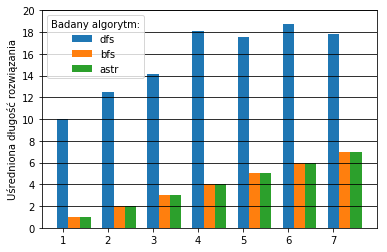
\includegraphics[width=1.1\textwidth]{output_3_0.png}
    \end{minipage}\hfill
    \begin{minipage}{0.45\textwidth}
        \centering
        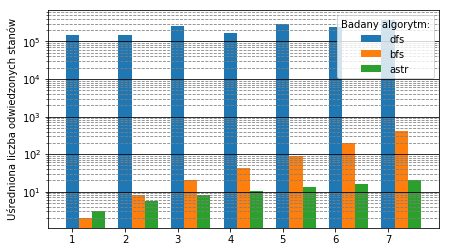
\includegraphics[width=1.1\textwidth]{output_3_1.png}
    \end{minipage}
}%
\end{figure}
\begin{figure}[H]
  \centering
  \makebox[\textwidth][c]{%
    \begin{minipage}{0.45\textwidth}
        \centering
        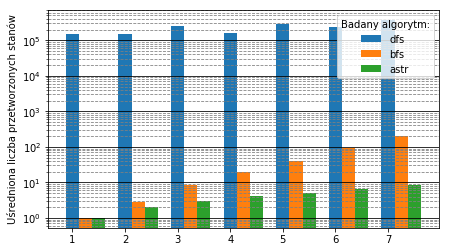
\includegraphics[width=1.1\textwidth]{output_3_2.png}
    \end{minipage}\hfill
    \begin{minipage}{0.45\textwidth}
        \centering
        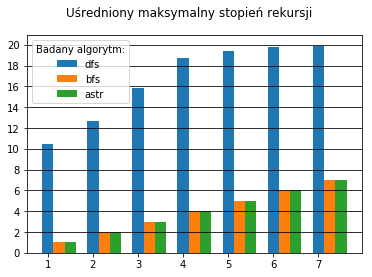
\includegraphics[width=1.1\textwidth]{output_3_3.png}
    \end{minipage}
}%
\end{figure}
\begin{figure}[H]
  \centering
    \begin{minipage}{0.45\textwidth}
        \centering
        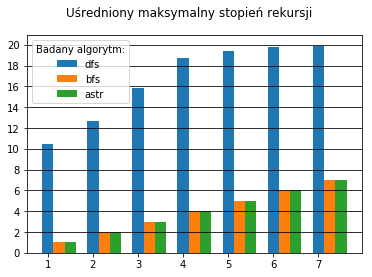
\includegraphics[width=1.1\textwidth]{output_3_3.png}
    \end{minipage}
\end{figure}

%end all algorithms

%bfs comp
\afterpage{
\thispagestyle{empty}
\begin{figure}[H]
  \centering
  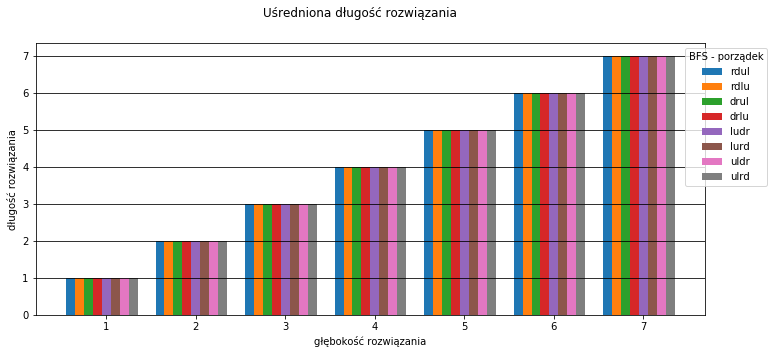
\includegraphics[scale=0.735]{output_5_0.png}
  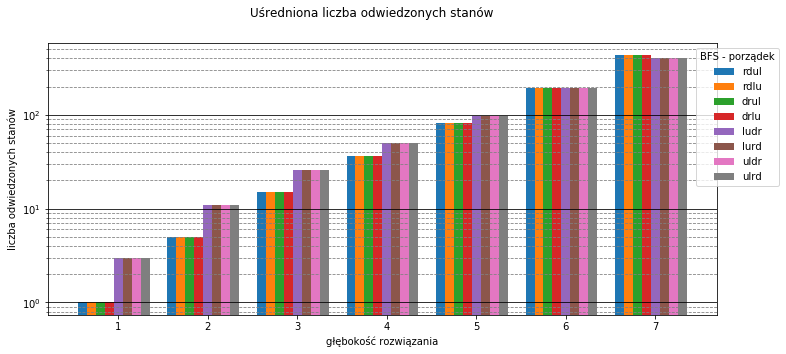
\includegraphics[scale=0.735]{output_5_1.png}
  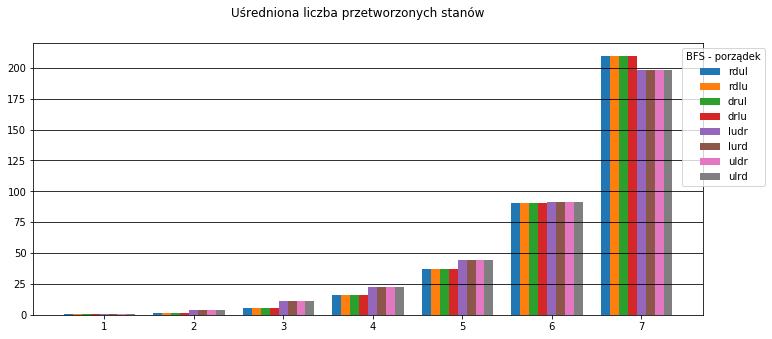
\includegraphics[scale=0.735]{output_5_2.png}
\end{figure}
}
\begin{figure}[H]
  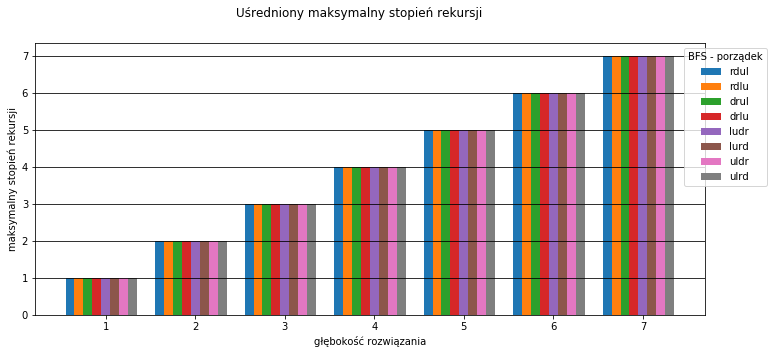
\includegraphics[scale=0.735]{output_5_3.png}
  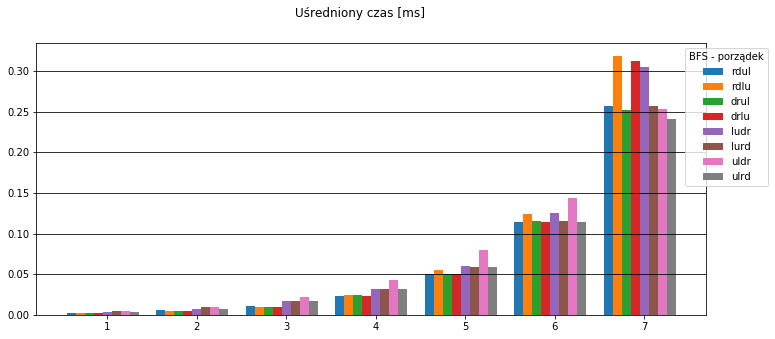
\includegraphics[scale=0.735]{output_5_4.png}
\end{figure}
%end bfs comp

%dfs comp
\afterpage{
\thispagestyle{empty}
\begin{figure}[H]
  \centering
  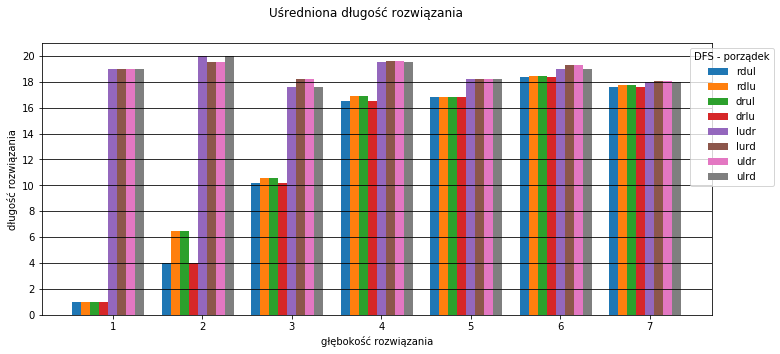
\includegraphics[scale=0.735]{output_6_0.png}
  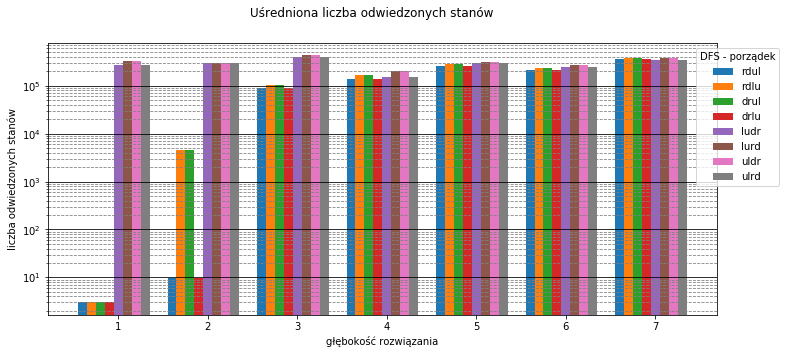
\includegraphics[scale=0.735]{output_6_1.png}
  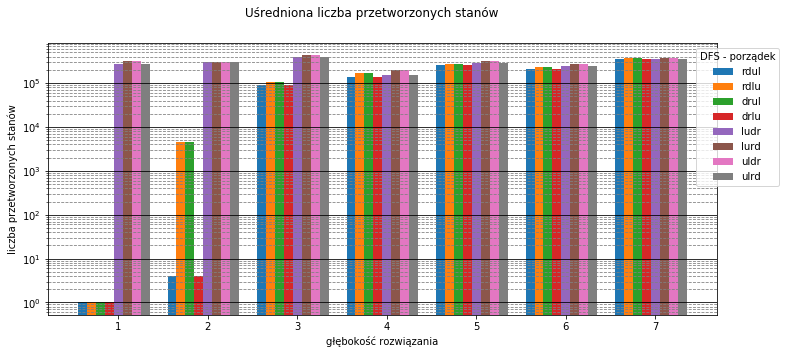
\includegraphics[scale=0.735]{output_6_2.png}
\end{figure}
}
\begin{figure}[H]
  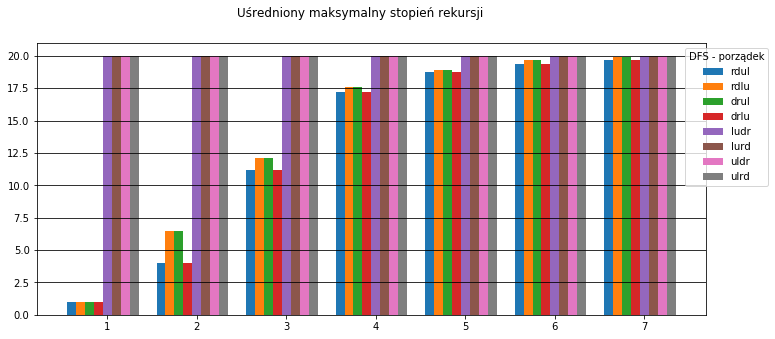
\includegraphics[scale=0.735]{output_6_3.png}
  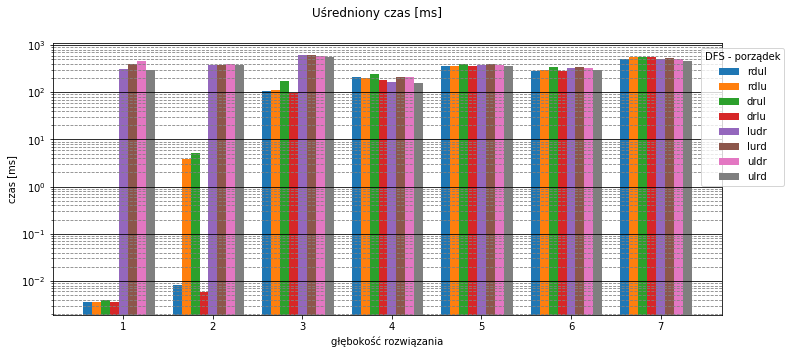
\includegraphics[scale=0.735]{output_6_4.png}
\end{figure}
%end dfs comp

%astr metrics comp
\begin{figure}[H]
  \centering
  \makebox[\textwidth][c]{%
    \begin{minipage}{0.45\textwidth}
        \centering
        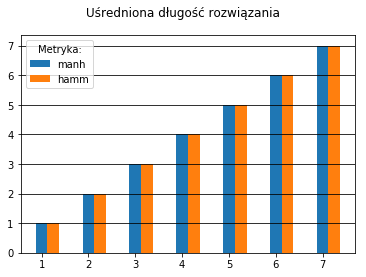
\includegraphics[width=1.1\textwidth]{output_4_0.png}
    \end{minipage}\hfill
    \begin{minipage}{0.45\textwidth}
        \centering
        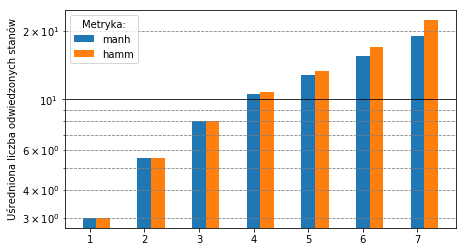
\includegraphics[width=1.1\textwidth]{output_4_1.png}
    \end{minipage}
}%
\end{figure}
\begin{figure}[H]
  \centering
  \makebox[\textwidth][c]{%
    \begin{minipage}{0.45\textwidth}
        \centering
        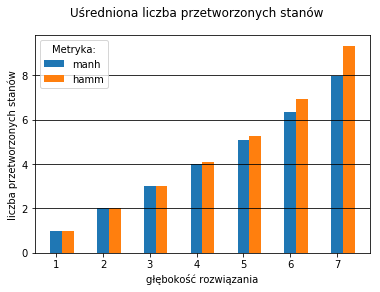
\includegraphics[width=1.1\textwidth]{output_4_2.png}
    \end{minipage}\hfill
    \begin{minipage}{0.45\textwidth}
        \centering
        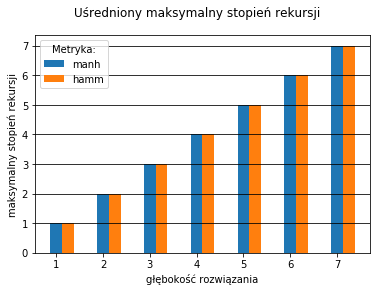
\includegraphics[width=1.1\textwidth]{output_4_3.png}
    \end{minipage}
}%
\end{figure}
\begin{figure}[H]
  \centering
    \begin{minipage}{0.45\textwidth}
        \centering
        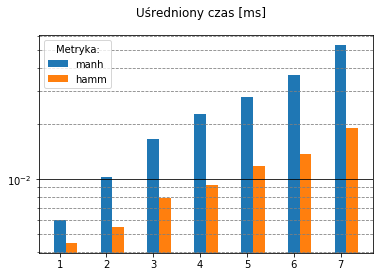
\includegraphics[width=1.1\textwidth]{output_4_4.png}
    \end{minipage}
\end{figure}
%end astr metrics comp

\restoregeometry

\end{document}
